\documentclass[9pt]{beamer}
\usetheme{metropolis}
\usepackage{amsmath}
\usepackage{amssymb}
\usepackage{graphicx}
\usepackage{booktabs}
\usepackage{xcolor}
\usepackage{tikz}
\usetikzlibrary{arrows,positioning,shapes.geometric,calc}

% Define color palette matching our project design system
\definecolor{primary}{HTML}{1abc9c}    % Deep Teal
\definecolor{secondary}{HTML}{3498db}  % Astro Blue
\definecolor{darkbg}{HTML}{2c3e50}     % Slate Blue
\definecolor{accent}{HTML}{e67e22}     % Orange

\setbeamercolor{palette primary}{bg=darkbg, fg=white}
\setbeamercolor{palette secondary}{bg=primary, fg=white}
\setbeamercolor{palette tertiary}{bg=secondary, fg=white}
\setbeamercolor{structure}{fg=primary}
\setbeamercolor{alerted text}{fg=accent}

\title{Foundations of Neural Networks \& Machine Learning}
\subtitle{A Comprehensive Tutorial: From Data Preprocessing to Classifier Interpretability}
\author{Astronomy Club}
\date{\today}

\begin{document}

\maketitle

% Slide 2: Table of Contents / Modules
\begin{frame}{Tutorial Roadmap}
  This tutorial covers the complete pipeline of machine learning classifiers, starting from raw tabular physical measurements to interpreting black-box neural networks:
  \begin{description}
    \item[Module 1:] \textbf{Data Preprocessing \& Feature Scaling}
      \begin{itemize}
        \item Physical scales, Standardization vs. Normalization, and train-test scaling isolation.
      \end{itemize}
    \item[Module 2:] \textbf{Neural Network Architecture \& Forward Propagation}
      \begin{itemize}
        \item The artificial neuron, hidden layers, matrix mechanics, and activation functions.
      \end{itemize}
    \item[Module 3:] \textbf{Multiclass Classification \& Loss Functions}
      \begin{itemize}
        \item Softmax normalization, Categorical Cross-Entropy, and loss math.
      \end{itemize}
    \item[Module 4:] \textbf{Backpropagation \& Optimization Math}
      \begin{itemize}
        \item Calculus chain rule, logit gradient derivations, and L2 weight decay.
      \end{itemize}
    \item[Module 5:] \textbf{Generalization & Hyperparameter Search}
      \begin{itemize}
        \item Data leakage, Stratification, K-Fold Cross-Validation, and Grid Search.
      \end{itemize}
    \item[Module 6:] \textbf{Model Diagnostics \& Interpretability}
      \begin{itemize}
        \item Multiclass metrics (F1, ROC, confusion matrices) and Permutation Importance.
      \end{itemize}
  \end{description}
\end{frame}

% Module 1 Header
\begin{frame}[plain]
  \vfill
  \centering
  \begin{beamercolorbox}[sep=8pt,center,shadow=true,rounded=true]{palette primary}
    \usebeamerfont{title}\textbf{Module 1: Data Preprocessing \& Feature Scaling}
  \end{beamercolorbox}
  \vfill
\end{frame}

% Slide 4: Why Scale Data?
\begin{frame}{Why Do We Scale Data?}
  In astronomical and physical datasets, different features represent distinct physical quantities and vary across vastly different numerical scales:
  \begin{itemize}
    \item \textbf{Redshift ($z$):} Typically a small decimal number, e.g., $z \in [0.01, 0.5]$ in local surveys.
    \item \textbf{Stellar Mass ($\log_{10} M_\star$):} Logarithmic solar mass units, e.g., $\log_{10} M_\star \in [8.0, 12.0]$ ($10^8$ to $10^{12} M_\odot$).
    \item \textbf{Star Formation Rate (SFR):} Logarithmic units, e.g., $\log_{10} \text{SFR} \in [-5.0, 2.0]$.
  \end{itemize}
  \begin{alertblock}{The Mathematical Hazard of Raw Features}
    If we feed unscaled features into gradient-based optimizers (like neural networks):
    \begin{enumerate}
      \item Features with larger absolute scales (like Stellar Mass) will dominate the weight updates.
      \item The loss surface will become highly elongated and anisotropic (stretched like a deep valley).
      \item Gradient descent will oscillate wildly, requiring an extremely small learning rate to avoid exploding gradients, leading to extremely slow convergence.
    \end{enumerate}
  \end{alertblock}
\end{frame}

% Slide 5: Standardization vs. Normalization
\begin{frame}{Standardization vs. Normalization}
  There are two primary methods for scaling physical features before feeding them to classifiers:
  \begin{description}
    \item[Normalization (Min-Max Scaling):]
      Rescales features linearly to fit within a fixed range, typically $[0, 1]$:
      $$x_{\text{norm}} = \frac{x - x_{\text{min}}}{x_{\text{max}} - x_{\text{min}}}$$
      \begin{itemize}
        \item \alert{Drawback:} Highly sensitive to outliers. A single extreme outlier (e.g., a hyper-luminous quasar) compresses the normal galaxy population into a tiny, indistinguishable range.
      \end{itemize}
    \item[Standardization (Z-Score Scaling):]
      Centers the feature to have a mean of $0$ and scales it to have a standard deviation of $1$:
      $$x_{\text{scaled}} = \frac{x - \mu}{\sigma}$$
      where $\mu$ is the mean and $\sigma$ is the standard deviation.
      \begin{itemize}
        \item \alert{Advantage:} Robust to outliers. Preserves the relative variance of features and ensures zero-centered symmetric input distributions, which aids gradient descent.
      \end{itemize}
  \end{description}
\end{frame}

% Slide 6: Hand-Worked Preprocessing Example
\begin{frame}{Hand-Worked Preprocessing Example}
  Let's standardize the Stellar Mass ($\log_{10} M_\star$) feature for a sample of $N=3$ host galaxies:
  $$\mathbf{x} = [9.0, 10.0, 11.0]^T \quad (\text{in units of } \log_{10} M_\odot)$$
  \begin{enumerate}
    \item \textbf{Step 1: Compute the sample mean ($\mu$):}
      $$\mu = \frac{1}{N} \sum_{i=1}^N x_i = \frac{9.0 + 10.0 + 11.0}{3} = 10.0$$
    \item \textbf{Step 2: Compute the sample standard deviation ($\sigma$):}
      $$\sigma = \sqrt{\frac{1}{N} \sum_{i=1}^N (x_i - \mu)^2} = \sqrt{\frac{(9-10)^2 + (10-10)^2 + (11-10)^2}{3}} = \sqrt{\frac{1 + 0 + 1}{3}} \approx 0.8165$$
    \item \textbf{Step 3: Standardize each data point ($x_{\text{scaled}} = \frac{x - \mu}{\sigma}$):}
      \begin{itemize}
        \item $x_1 = 9.0 \implies x_{\text{scaled}, 1} = \frac{9.0 - 10.0}{0.8165} \approx -1.225$
        \item $x_2 = 10.0 \implies x_{\text{scaled}, 2} = \frac{10.0 - 10.0}{0.8165} = 0.0$
        \item $x_3 = 11.0 \implies x_{\text{scaled}, 3} = \frac{11.0 - 10.0}{0.8165} \approx +1.225$
      \end{itemize}
  \end{enumerate}
  The resulting standardized vector $\mathbf{x}_{\text{scaled}} \approx [-1.225, 0.0, 1.225]^T$ now has a mean of $0$ and variance of $1$.
\end{frame}

% Slide 7: Preprocessing Pitfalls: Train-Test Scaling Isolation
\begin{frame}{Preprocessing Pitfalls: Train-Test Scaling Isolation}
  When preparing data for evaluation, we split the dataset into a training set and a testing set. Scaling must be applied with extreme caution.
  \begin{alertblock}{The Scaling Leakage Trap}
    A common mistake is scaling the entire dataset before splitting, or fitting the scaler on the test set. 
    If test set samples are used to compute the mean $\mu$ and standard deviation $\sigma$, statistical information about the test set's distribution leaks into the training phase. This is a form of data leakage.
  \end{alertblock}
  \begin{block}{The Fit-Transform Boundary Rule}
    To maintain strict validation boundaries:
    \begin{enumerate}
      \item \textbf{Fit only on Training Data:} Compute $\mu_{\text{train}}$ and $\sigma_{\text{train}}$ exclusively using the training set.
      \item \textbf{Transform both partitions:} Scale the training set using training statistics, and scale the test set using those same training statistics ($\mu_{\text{train}}$ and $\sigma_{\text{train}}$).
    \end{enumerate}
    $$X_{\text{train, scaled}} = \frac{X_{\text{train}} - \mu_{\text{train}}}{\sigma_{\text{train}}}, \quad X_{\text{test, scaled}} = \frac{X_{\text{test}} - \mu_{\text{train}}}{\sigma_{\text{train}}}$$
  \end{block}
\end{frame}

% Module 2 Header
\begin{frame}[plain]
  \vfill
  \centering
  \begin{beamercolorbox}[sep=8pt,center,shadow=true,rounded=true]{palette primary}
    \usebeamerfont{title}\textbf{Module 2: Neural Network Architecture \& Forward Propagation}
  \end{beamercolorbox}
  \vfill
\end{frame}

% Slide 9: Biological Inspiration & The Artificial Neuron
\begin{frame}{Biological Inspiration \& The Artificial Neuron}
  Neural networks are inspired by the brain's network of biological neurons, which receive electrical signals, integrate them, and fire once a voltage threshold is passed.
  \begin{block}{The Artificial Neuron (Node)}
    An artificial neuron is a mathematical node that:
    \begin{enumerate}
      \item Receives a set of numerical inputs: $\mathbf{x} = [x_0, x_1, \dots, x_d]^T$.
      \item Multiplies each input by a corresponding weight parameter: $\mathbf{w} = [w_0, w_1, \dots, w_d]^T$.
      \item Integrates the weighted inputs and adds a bias parameter $b$:
        $$z = \sum_{i=1}^d w_i x_i + b = \mathbf{w}^T \mathbf{x} + b$$
      \item Applies a non-linear activation function $f(z)$ to produce the output activation $a$:
        $$a = f(z) = f(\mathbf{w}^T \mathbf{x} + b)$$
    \end{enumerate}
  \end{block}
\end{frame}

% Slide 10: Single Neuron Illustration
\begin{frame}{Illustration: The Artificial Neuron Model}
  Below is a schematic of a single neuron. The inputs are weighted, summed with a bias, and passed through an activation function to generate the output:
  \vfill
  \centering
  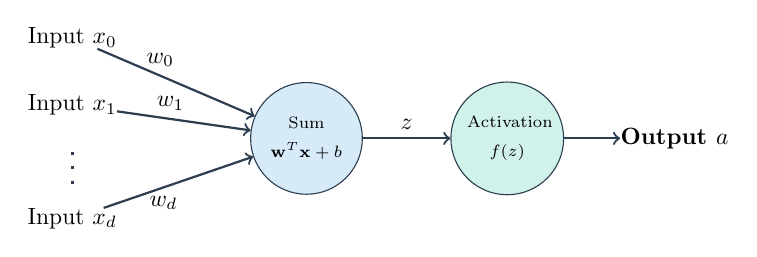
\begin{tikzpicture}[draw=darkbg, scale=0.85, every node/.style={transform shape}]
    % Sum junction
    \node[circle, draw, fill=secondary!20, minimum size=1.4cm, text width=1.2cm, align=center] (sum) at (2,0) {\scriptsize Sum \\ $\mathbf{w}^T\mathbf{x} + b$};
    % Activation
    \node[circle, draw, fill=primary!20, minimum size=1.4cm, text width=1.2cm, align=center] (act) at (5,0) {\scriptsize Activation \\ $f(z)$};
    % Output
    \node[inner sep=0pt] (out) at (7.5,0) {\textbf{Output $a$}};
    
    % Inputs
    \node[inner sep=0pt] (x0) at (-1.5,1.5) {Input $x_0$};
    \node[inner sep=0pt] (x1) at (-1.5,0.5) {Input $x_1$};
    \node[inner sep=0pt] (xd) at (-1.5,-1.2) {Input $x_d$};
    
    % Connections
    \draw[->, thick, draw=darkbg] (x0) -- node[above, pos=0.4] {$w_0$} (sum);
    \draw[->, thick, draw=darkbg] (x1) -- node[above, pos=0.4] {$w_1$} (sum);
    \draw[loosely dotted, very thick, draw=darkbg] (-1.5,-0.2) -- (-1.5,-0.8);
    \draw[->, thick, draw=darkbg] (xd) -- node[below, pos=0.4] {$w_d$} (sum);
    
    \draw[->, thick, draw=darkbg] (sum) -- node[above] {$z$} (act);
    \draw[->, thick, draw=darkbg] (act) -- (out);
  \end{tikzpicture}
  \vfill
\end{frame}

% Slide 11: Going Deeper: Multi-Layer Perceptrons (MLPs)
\begin{frame}{Going Deeper: Multi-Layer Perceptrons (MLPs)}
  A single neuron can only resolve linear decision boundaries (hyperplanes). To learn complex, curved boundaries, we stack neurons in layers, forming a \textbf{Multi-Layer Perceptron (MLP)}:
  \begin{itemize}
    \item \textbf{Input Layer ($l=0$):} Represents the scaled input features. No computations occur here.
    \item \textbf{Hidden Layers ($l = 1 \dots L-1$):} Intermediate layers that extract higher-level representations. The output of one layer serves as the input to the next.
    \item \textbf{Output Layer ($l=L$):} The final layer, which produces logits or predictions.
  \end{itemize}
  An MLP is \textbf{fully connected} (or dense), meaning every neuron in layer $l$ receives inputs from every single neuron in the preceding layer $l-1$.
\end{frame}

% Slide 12: MLP Network Graph Illustration
\begin{frame}{Illustration: 3-Layer MLP Feedforward Network}
  Below is a fully connected neural network with 4 inputs ($d=4$), a hidden layer with 5 neurons ($H=5$), and 3 output nodes ($C=3$):
  \vfill
  \centering
  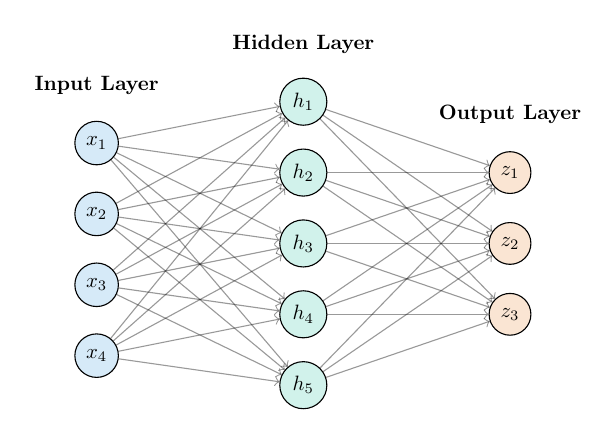
\begin{tikzpicture}[scale=0.75, every node/.style={transform shape}]
    % Input nodes
    \foreach \i in {1,...,4} {
      \node[circle, draw, fill=secondary!20, minimum size=0.6cm] (in-\i) at (0, 3.5-\i*1.2) {$x_\i$};
    }
    % Hidden nodes
    \foreach \j in {1,...,5} {
      \node[circle, draw, fill=primary!20, minimum size=0.6cm] (hid-\j) at (3.5, 4.2-\j*1.2) {$h_\j$};
    }
    % Output nodes
    \foreach \k in {1,...,3} {
      \node[circle, draw, fill=accent!20, minimum size=0.6cm] (out-\k) at (7, 3.0-\k*1.2) {$z_\k$};
    }
    
    % Connect inputs to hidden
    \foreach \i in {1,...,4} {
      \foreach \j in {1,...,5} {
        \draw[->, thin, opacity=0.4] (in-\i) -- (hid-\j);
      }
    }
    % Connect hidden to outputs
    \foreach \j in {1,...,5} {
      \foreach \k in {1,...,3} {
        \draw[->, thin, opacity=0.4] (hid-\j) -- (out-\k);
      }
    }
    
    \node[above] at (0, 3.0) {\textbf{Input Layer}};
    \node[above] at (3.5, 3.7) {\textbf{Hidden Layer}};
    \node[above] at (7, 2.5) {\textbf{Output Layer}};
  \end{tikzpicture}
  \vfill
\end{frame}

% Slide 13: MLP Feedforward Mathematics
\begin{frame}{MLP Feedforward Mathematics}
  To evaluate the network, we compute the activations of each layer sequentially from left to right. For any layer $l \ge 1$:
  $$\mathbf{z}^{(l)} = \mathbf{W}^{(l)} \mathbf{a}^{(l-1)} + \mathbf{b}^{(l)}$$
  $$\mathbf{a}^{(l)} = f(\mathbf{z}^{(l)})$$
  Where:
  \begin{itemize}
    \item $\mathbf{a}^{(l-1)}$ is the activation vector from the previous layer ($\mathbf{a}^{(0)} = \mathbf{x}_{\text{scaled}}$).
    \item $\mathbf{W}^{(l)}$ is the weight matrix of layer $l$, where element $W_{ij}^{(l)}$ represents the weight connecting neuron $j$ in layer $l-1$ to neuron $i$ in layer $l$.
    \item $\mathbf{b}^{(l)}$ is the bias vector of layer $l$.
    \item $f(\cdot)$ is the activation function, applied element-wise.
  \end{itemize}
  This vectorization allows us to leverage highly optimized BLAS (Basic Linear Algebra Subprograms) libraries for matrix operations.
\end{frame}

% Slide 14: Hidden Layer Weights and Biases Dimension Analysis
\begin{frame}{Weight and Bias Dimension Analysis}
  Understanding matrix dimensions is essential for debugging neural network architectures. Let's analyze a network with:
  $$\text{Inputs } d=4, \quad \text{Hidden Layer Sizes } = (32, 16), \quad \text{Outputs } C=3$$
  \begin{description}
    \item[Layer 1 (First Hidden Layer):]
      \begin{itemize}
        \item Receives input $\mathbf{a}^{(0)} \in \mathbb{R}^4$. Outputs activation $\mathbf{a}^{(1)} \in \mathbb{R}^{32}$.
        \item Weight matrix $\mathbf{W}^{(1)}$ must map $\mathbb{R}^4 \to \mathbb{R}^{32}$: $\quad \mathbf{W}^{(1)} \in \mathbb{R}^{32 \times 4}$.
        \item Bias vector matches output size: $\quad \mathbf{b}^{(1)} \in \mathbb{R}^{32}$.
      \end{itemize}
    \item[Layer 2 (Second Hidden Layer):]
      \begin{itemize}
        \item Receives input $\mathbf{a}^{(1)} \in \mathbb{R}^{32}$. Outputs activation $\mathbf{a}^{(2)} \in \mathbb{R}^{16}$.
        \item Weight matrix $\mathbf{W}^{(2)}$ maps $\mathbb{R}^{32} \to \mathbb{R}^{16}$: $\quad \mathbf{W}^{(2)} \in \mathbb{R}^{16 \times 32}$.
        \item Bias vector matches output size: $\quad \mathbf{b}^{(2)} \in \mathbb{R}^{16}$.
      \end{itemize}
    \item[Layer 3 (Output Layer):]
      \begin{itemize}
        \item Receives input $\mathbf{a}^{(2)} \in \mathbb{R}^{16}$. Outputs logits $\mathbf{z}^{(3)} \in \mathbb{R}^3$.
        \item Weight matrix $\mathbf{W}^{(3)}$ maps $\mathbb{R}^{16} \to \mathbb{R}^3$: $\quad \mathbf{W}^{(3)} \in \mathbb{R}^{3 \times 16}$.
        \item Bias vector matches output size: $\quad \mathbf{b}^{(3)} \in \mathbb{R}^3$.
      \end{itemize}
  \end{description}
\end{frame}

% Slide 15: The Necessity of Non-Linear Activations
\begin{frame}{The Necessity of Non-Linear Activations}
  What happens if we remove the non-linear activation functions $f(z)$ and let $f(z) = z$?
  \begin{block}{Collapsing Layers Proof}
    Consider a two-layer linear MLP with inputs $\mathbf{x}$, weights $\mathbf{W}^{(1)}, \mathbf{W}^{(2)}$ and biases $\mathbf{b}^{(1)}, \mathbf{b}^{(2)}$:
    $$\mathbf{a}^{(1)} = \mathbf{W}^{(1)} \mathbf{x} + \mathbf{b}^{(1)}$$
    $$\mathbf{y}_{\text{pred}} = \mathbf{W}^{(2)} \mathbf{a}^{(1)} + \mathbf{b}^{(2)}$$
    Substituting the first equation into the second:
    $$\mathbf{y}_{\text{pred}} = \mathbf{W}^{(2)} \left( \mathbf{W}^{(1)} \mathbf{x} + \mathbf{b}^{(1)} \right) + \mathbf{b}^{(2)}$$
    $$\mathbf{y}_{\text{pred}} = \left( \mathbf{W}^{(2)} \mathbf{W}^{(1)} \right) \mathbf{x} + \left( \mathbf{W}^{(2)} \mathbf{b}^{(1)} + \mathbf{b}^{(2)} \right)$$
    Let $\mathbf{W}' = \mathbf{W}^{(2)} \mathbf{W}^{(1)}$ and $\mathbf{b}' = \mathbf{W}^{(2)} \mathbf{b}^{(1)} + \mathbf{b}^{(2)}$. Then:
    $$\mathbf{y}_{\text{pred}} = \mathbf{W}' \mathbf{x} + \mathbf{b}'$$
  \end{block}
  This collapses into a single-layer linear regression! Stacking linear layers adds zero representation power. Non-linear activations are required to bend and curve boundaries.
\end{frame}

% Slide 16: Activation Function: ReLU
\begin{frame}{Activation Function: ReLU}
  The \textbf{Rectified Linear Unit (ReLU)} is the most widely used activation function in modern deep learning:
  $$f(z) = \max(0, z)$$
  \begin{columns}
    \begin{column}{0.5\textwidth}
      \begin{itemize}
        \item \textbf{Output Range:} $[0, \infty)$
        \item \textbf{Derivative:}
          $$f'(z) = \begin{cases} 1 & \text{if } z > 0 \\ 0 & \text{if } z < 0 \end{cases}$$
        \item \textbf{Pros:}
          \begin{itemize}
            \item Extremely fast to calculate (requires only a maximum check).
            \item The derivative is $1.0$ for all positive inputs, preventing vanishing gradients during backpropagation.
          \end{itemize}
      \end{itemize}
    \end{column}
    \begin{column}{0.5\textwidth}
      \begin{itemize}
        \item \textbf{Cons:}
          \begin{itemize}
            \item Not zero-centered.
            \item \alert{Dying ReLU Problem:} If a neuron receives updates that make it negative for all training points, its gradient becomes exactly zero. It will never fire again, becoming a dead weight in the network.
          \end{itemize}
      \end{itemize}
    \end{column}
  \end{columns}
\end{frame}

% Slide 17: Activation Function: Tanh
\begin{frame}{Activation Function: Tanh}
  The \textbf{Hyperbolic Tangent (tanh)} activation function is a smooth, S-shaped curve:
  $$f(z) = \tanh(z) = \frac{e^z - e^{-z}}{e^z + e^{-z}}$$
  \begin{columns}
    \begin{column}{0.5\textwidth}
      \begin{itemize}
        \item \textbf{Output Range:} $(-1, 1)$
        \item \textbf{Derivative:}
          $$f'(z) = 1 - \tanh^2(z)$$
        \item \textbf{Pros:}
          \begin{itemize}
            \item Outputs are \textbf{zero-centered} (mean output is close to 0). This centers the activations for subsequent layers, which speeds up convergence.
          \end{itemize}
      \end{itemize}
    \end{column}
    \begin{column}{0.5\textwidth}
      \begin{itemize}
        \item \textbf{Cons:}
          \begin{itemize}
            \item Computationally heavier due to exponentiations.
            \item \alert{Vanishing Gradient Problem:} For large positive or negative inputs, $\tanh(z)$ saturates close to $+1$ or $-1$. In these regions, the derivative $f'(z) \approx 0$, which stops gradient flow during training.
          \end{itemize}
      \end{itemize}
    \end{column}
  \end{columns}
\end{frame}

% Module 3 Header
\begin{frame}[plain]
  \vfill
  \centering
  \begin{beamercolorbox}[sep=8pt,center,shadow=true,rounded=true]{palette primary}
    \usebeamerfont{title}\textbf{Module 3: Multi-Class Output \& Loss Functions}
  \end{beamercolorbox}
  \vfill
\end{frame}

% Slide 19: Multiclass Classification: Logits vs. Probabilities
\begin{frame}{Multiclass Classification: Logits vs. Probabilities}
  In multiclass classification (e.g., classifying a galaxy as Class 0: Background, Class 1: CC-SN host, or Class 2: Ia-SN host), the output layer has $C=3$ neurons.
  \begin{itemize}
    \item The raw real-valued output vector of the final layer is called the \textbf{logits} vector:
      $$\mathbf{z} = [z_0, z_1, \dots, z_{C-1}]^T \in \mathbb{R}^C$$
    \item Logits are unbounded: they can be negative, positive, or zero, and they do not sum to $1$.
    \item In physics and classification, we need a vector of probabilities:
      $$\mathbf{P} = [P_0, P_1, \dots, P_{C-1}]^T$$
      where each $P_c \in [0, 1]$ represents the probability that the galaxy belongs to class $c$, and:
      $$\sum_{c=0}^{C-1} P_c = 1.0$$
  \end{itemize}
\end{frame}

% Slide 20: The Softmax Normalization Function
\begin{frame}{The Softmax Normalization Function}
  To convert raw logits $\mathbf{z}$ into a valid probability distribution, we apply the \textbf{Softmax function}:
  $$P_c = P(y = c \mid \mathbf{x}) = \frac{e^{z_c}}{\sum_{j=0}^{C-1} e^{z_j}}$$
  \begin{block}{Why do we exponentiate?}
    \begin{enumerate}
      \item \textbf{Enforces Positivity:} Exponentiating $e^{z_c} > 0$ ensures all probabilities are strictly positive, even if a logit $z_c$ is highly negative.
      \item \textbf{Enforces Sum-to-One:} Dividing by the sum of all exponentiated logits ensures that $\sum_c P_c = 1.0$ exactly.
      \item \textbf{Highlights the Max:} Exponentiating accentuates differences: the largest logit receives a disproportionately higher probability, making the model's predictions more decisive.
    \end{enumerate}
  \end{block}
\end{frame}

% Slide 21: Hand-Worked Softmax Example
\begin{frame}{Hand-Worked Softmax Example}
  Let's calculate the predicted probabilities for a galaxy that yields raw output logits:
  $$\mathbf{z} = [-0.5, 1.5, 0.0]^T$$
  representing Class 0 (Background), Class 1 (CC-SN), and Class 2 (Ia-SN).
  \begin{enumerate}
    \item \textbf{Step 1: Compute the exponentiated logits ($e^{z_c}$):}
      \begin{itemize}
        \item $e^{z_0} = e^{-0.5} \approx 0.6065$
        \item $e^{z_1} = e^{1.5} \approx 4.4817$
        \item $e^{z_2} = e^{0.0} = 1.0000$
      \end{itemize}
    \item \textbf{Step 2: Compute the sum of exponentiated logits (denominator):}
      $$\sum_{j=0}^{2} e^{z_j} = 0.6065 + 4.4817 + 1.0000 = 6.0882$$
    \item \textbf{Step 3: Divide each exponentiated logit by the sum:}
      \begin{itemize}
        \item $P_0 = 0.6065 / 6.0882 \approx \mathbf{0.100}$ (10.0\%)
        \item $P_1 = 4.4817 / 6.0882 \approx \mathbf{0.736}$ (73.6\%)
        \item $P_2 = 1.0000 / 6.0882 \approx \mathbf{0.164}$ (16.4\%)
      \end{itemize}
  \end{enumerate}
  The output probability vector is $\mathbf{P} \approx [0.100, 0.736, 0.164]^T$. The network predicts Class 1 with $73.6\%$ confidence.
\end{frame}

% Slide 22: Loss Functions: Why Not Mean Squared Error (MSE)?
\begin{frame}{Loss Functions: Why Not Mean Squared Error (MSE)?}
  To train a classifier, we need a loss function $\mathcal{L}$ that measures the error between predictions $\mathbf{P}$ and true labels $\mathbf{y}$.
  \begin{itemize}
    \item Why don't we use the standard Mean Squared Error (MSE) from regression?
      $$\mathcal{L}_{\text{MSE}} = \frac{1}{C} \sum_{c=0}^{C-1} (P_c - y_c)^2$$
  \end{itemize}
  \begin{alertblock}{Problems with MSE for Classification}
    \begin{enumerate}
      \item \textbf{Non-Convexity:} Combining MSE with Softmax or Sigmoid functions creates a highly non-convex loss surface with many local minima.
      \item \textbf{Vanishing Gradients:} If a model makes a highly confident incorrect prediction (e.g., $P_c \approx 0$ when true label is $1$), the gradient of MSE with respect to the input weights becomes extremely small. The network will get stuck and stop learning.
    \end{enumerate}
  \end{alertblock}
\end{frame}

% Slide 23: Categorical Cross-Entropy Loss
\begin{frame}{Categorical Cross-Entropy Loss}
  For multiclass classification, the standard objective function is the \textbf{Categorical Cross-Entropy Loss}:
  \begin{block}{Loss for a single instance $i$}
    $$\mathcal{L}_i = - \sum_{c=0}^{C-1} y_c \log P_c$$
    where $y_c$ is a one-hot encoded representation of the true label:
    $$y_c = \begin{cases} 1 & \text{if class } c \text{ is the true label} \\ 0 & \text{otherwise} \end{cases}$$
  \end{block}
  \begin{itemize}
    \item If the true class is $k$, then $y_k=1$ and all other $y_{c \neq k} = 0$. The formula simplifies to:
      $$\mathcal{L}_i = - \log P_k$$
    \item \textbf{Intuition:} We only care about maximizing the probability of the correct class.
      \begin{itemize}
        \item If $P_k \to 1.0$, the loss $\mathcal{L}_i \to - \log(1) = 0$.
        \item If $P_k \to 0.0$, the loss $\mathcal{L}_i \to - \log(0) = \infty$, heavily penalizing incorrect predictions.
      \end{itemize}
  \end{itemize}
\end{frame}

% Slide 24: Hand-Worked Cross-Entropy Example
\begin{frame}{Hand-Worked Cross-Entropy Example}
  Let's calculate the Cross-Entropy loss for a galaxy with the following parameters:
  \begin{itemize}
    \item \textbf{True Label:} Class 1 (CC-SN host). In one-hot encoding:
      $$\mathbf{y} = [0, 1, 0]^T$$
    \item \textbf{Predicted Probabilities:} From our Softmax calculations:
      $$\mathbf{P} = [0.100, 0.736, 0.164]^T$$
  \end{itemize}
  \begin{block}{Loss Computation}
    Applying the Categorical Cross-Entropy formula:
    \begin{align*}
      \mathcal{L} &= - \sum_{c=0}^{2} y_c \log P_c \\
      &= - \left( y_0 \log P_0 + y_1 \log P_1 + y_2 \log P_2 \right) \\
      &= - \left( 0 \cdot \log(0.100) + 1 \cdot \log(0.736) + 0 \cdot \log(0.164) \right) \\
      &= - \log(0.736) \\
      &\approx - (-0.3065) \approx \mathbf{0.3065}
    \end{align*}
    If the predicted probability for the true class was lower, e.g., $P_1 = 0.20$, the loss would be $- \log(0.20) \approx 1.609$, which is much higher.
  \end{block}
\end{frame}

% Module 4 Header
\begin{frame}[plain]
  \vfill
  \centering
  \begin{beamercolorbox}[sep=8pt,center,shadow=true,rounded=true]{palette primary}
    \usebeamerfont{title}\textbf{Module 4: Backpropagation \& Optimization Math}
  \end{beamercolorbox}
  \vfill
\end{frame}

% Slide 26: How Networks Learn: Gradient Descent
\begin{frame}{How Networks Learn: Gradient Descent}
  A neural network is trained by finding weights $\mathbf{W}$ and biases $\mathbf{b}$ that minimize the average loss across all $N$ training samples:
  $$\mathcal{L} = \frac{1}{N} \sum_{i=1}^N \mathcal{L}_i$$
  We update the weight parameters using \textbf{Gradient Descent}:
  $$\mathbf{W}^{(l)} \leftarrow \mathbf{W}^{(l)} - \eta \frac{\partial \mathcal{L}}{\partial \mathbf{W}^{(l)}}$$
  where $\eta > 0$ is the learning rate.
  \begin{block}{Backpropagation}
    To compute the partial derivatives $\frac{\partial \mathcal{L}}{\partial \mathbf{W}^{(l)}}$ for every layer, we use the \textbf{Chain Rule of Calculus}, propagating the error gradients backward from the output layer to the input layer.
  \end{block}
\end{frame}

% Slide 27: Softmax Derivative Jacobian (Part 1 - Setup)
\begin{frame}{Softmax Derivative Jacobian (Part 1 - Setup)}
  Let's derive the derivative of the Softmax output $P_k$ with respect to the input logit $z_c$.
  Recall that $P_k = e^{z_k} / \sum_{j} e^{z_j}$. Let $\Sigma = \sum_{j} e^{z_j}$.
  Using the Quotient Rule:
  $$\left( \frac{u}{v} \right)' = \frac{u'v - uv'}{v^2}$$
  We set $u = e^{z_k}$ and $v = \Sigma$.
  \begin{itemize}
    \item The derivative of the denominator is:
      $$\frac{\partial \Sigma}{\partial z_c} = \frac{\partial}{\partial z_c} \sum_{j} e^{z_j} = e^{z_c}$$
    \item The derivative of the numerator $u = e^{z_k}$ depends on whether $k = c$:
      $$\frac{\partial e^{z_k}}{\partial z_c} = \delta_{kc} e^{z_k}$$
      where Kronecker's delta $\delta_{kc} = 1$ if $k=c$, and $0$ otherwise.
  \end{itemize}
\end{frame}

% Slide 28: Softmax Derivative Jacobian (Part 2 - Calculation)
\begin{frame}{Softmax Derivative Jacobian (Part 2 - Calculation)}
  Substituting these derivatives into the quotient rule:
  \begin{align*}
    \frac{\partial P_k}{\partial z_c} &= \frac{\left( \delta_{kc} e^{z_k} \right) \Sigma - e^{z_k} \left( e^{z_c} \right)}{\Sigma^2} \\
    &= \frac{\delta_{kc} e^{z_k}}{\Sigma} - \frac{e^{z_k} e^{z_c}}{\Sigma^2} \\
    &= \delta_{kc} \left( \frac{e^{z_k}}{\Sigma} \right) - \left( \frac{e^{z_k}}{\Sigma} \right) \left( \frac{e^{z_c}}{\Sigma} \right) \\
    &= \delta_{kc} P_k - P_k P_c \\
    &= P_k (\delta_{kc} - P_c)
  \end{align*}
  \begin{block}{Softmax Gradient Summary}
    \begin{itemize}
      \item If $k = c$ (diagonal elements): $\quad \frac{\partial P_c}{\partial z_c} = P_c (1 - P_c)$
      \item If $k \neq c$ (off-diagonal elements): $\quad \frac{\partial P_k}{\partial z_c} = - P_k P_c$
    \end{itemize}
  \end{block}
\end{frame}

% Slide 29: Cross-Entropy Loss Logit Gradient (Part 1 - Chain Rule)
\begin{frame}{Cross-Entropy Loss Logit Gradient (Part 1 - Chain Rule)}
  Now, let's derive the gradient of the single-galaxy Cross-Entropy loss $\mathcal{L}_i = - \sum_{k} y_k \log P_k$ with respect to the output logits $z_c$.
  Applying the Chain Rule:
  \begin{align*}
    \frac{\partial \mathcal{L}_i}{\partial z_c} &= - \sum_{k=0}^{C-1} y_k \frac{\partial \log P_k}{\partial z_c} \\
    &= - \sum_{k=0}^{C-1} y_k \frac{1}{P_k} \frac{\partial P_k}{\partial z_c}
  \end{align*}
  Now we substitute our Softmax Jacobian result $\frac{\partial P_k}{\partial z_c} = P_k (\delta_{kc} - P_c)$ into this equation.
\end{frame}

% Slide 30: Cross-Entropy Loss Logit Gradient (Part 2 - Derivation)
\begin{frame}{Cross-Entropy Loss Logit Gradient (Part 2 - Derivation)}
  Performing the substitution and simplifying:
  \begin{align*}
    \frac{\partial \mathcal{L}_i}{\partial z_c} &= - \sum_{k=0}^{C-1} y_k \frac{1}{P_k} \left[ P_k (\delta_{kc} - P_c) \right] \\
    &= - \sum_{k=0}^{C-1} y_k (\delta_{kc} - P_c) \\
    &= - \sum_{k=0}^{C-1} y_k \delta_{kc} + \sum_{k=0}^{C-1} y_k P_c \\
    &= - y_c + P_c \sum_{k=0}^{C-1} y_k
  \end{align*}
  Since $\mathbf{y}$ is a probability distribution (one-hot encoded), it sums to exactly $1.0$ ($\sum_{k} y_k = 1.0$).
  $$\frac{\partial \mathcal{L}_i}{\partial z_c} = P_c - y_c$$
  \begin{alertblock}{The Gradient Rule}
    The error gradient at the output logit is simply the linear difference between predicted probability and ground truth label: $P_c - y_c$.
  \end{alertblock}
\end{frame}

% Slide 31: Regularization: Overfitting & L2 Weight Decay
\begin{frame}{Regularization: Overfitting \& L2 Weight Decay}
  A neural network with many hidden units has high capacity and can easily overfit the training set, memorizing statistical noise rather than physical relationships.
  To prevent this, we add an \textbf{L2 Regularization penalty} (also known as weight decay) to the objective function:
  $$\mathcal{L} = \mathcal{L}_0 + \frac{\alpha}{2} \sum_{w} w^2$$
  where $\mathcal{L}_0$ is the standard unregularized cross-entropy loss, and $\alpha > 0$ is the regularization strength.
  \begin{block}{Gradient Update with Weight Decay}
    Taking the derivative with respect to a single weight $w$:
    $$\frac{\partial \mathcal{L}}{\partial w} = \frac{\partial \mathcal{L}_0}{\partial w} + \alpha w$$
    The gradient descent update rule becomes:
    $$w \leftarrow w - \eta \frac{\partial \mathcal{L}}{\partial w} = w - \eta \left( \frac{\partial \mathcal{L}_0}{\partial w} + \alpha w \right) = (1 - \eta \alpha) w - \eta \frac{\partial \mathcal{L}_0}{\partial w}$$
  \end{block}
  At each step, the weight is first shrunk by a factor $(1 - \eta \alpha) < 1.0$, penalizing large weights and encouraging simpler decision boundaries.
\end{frame}

% Module 5 Header
\begin{frame}[plain]
  \vfill
  \centering
  \begin{beamercolorbox}[sep=8pt,center,shadow=true,rounded=true]{palette primary}
    \usebeamerfont{title}\textbf{Module 5: Generalization \& Hyperparameter Search}
  \end{beamercolorbox}
  \vfill
\end{frame}

% Slide 33: Hyperparameters vs. Model Parameters
\begin{frame}{Hyperparameters vs. Model Parameters}
  When training classifiers, it is important to distinguish between two types of variables:
  \begin{description}
    \item[Model Parameters:]
      Weights ($\mathbf{W}$) and biases ($\mathbf{b}$). These are learned directly from the training data by minimizing the loss function via backpropagation.
    \item[Hyperparameters:]
      External settings configured before training begins. They control the training process and model structure, e.g.:
      \begin{itemize}
        \item Network architecture: number of hidden layers and layer widths.
        \item Activation functions: ReLU vs. tanh.
        \item Learning rate $\eta$ and training epoch count.
        \item Regularization strength $\alpha$ (weight decay).
      \end{itemize}
  \end{description}
  Hyperparameters cannot be learned via standard gradient descent. Instead, we must search across a hyperparameter grid to find the optimal configuration.
\end{frame}

% Slide 34: Validation Strategies: Train-Validation-Test Splits
\begin{frame}{Validation Strategies: Train-Validation-Test Splits}
  To evaluate hyperparameters, we partition our raw dataset:
  \begin{center}
    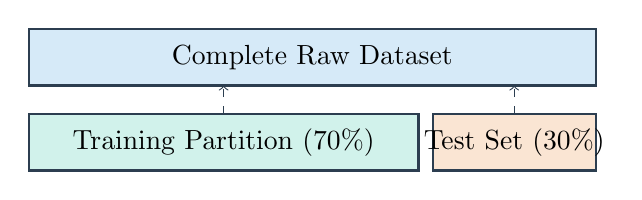
\begin{tikzpicture}[scale=0.9]
      \draw[draw=darkbg, fill=secondary!20, thick] (0,0) rectangle (8, 0.8);
      \node at (4, 0.4) {Complete Raw Dataset};
      
      \draw[draw=darkbg, fill=primary!20, thick] (0,-1.2) rectangle (5.5, -0.4);
      \node at (2.75, -0.8) {Training Partition (70\%)};
      
      \draw[draw=darkbg, fill=accent!20, thick] (5.7,-1.2) rectangle (8, -0.4);
      \node at (6.85, -0.8) {Test Set (30\%)};
      
      \draw[dashed, ->, draw=darkbg] (2.75,-0.4) -- (2.75,0);
      \draw[dashed, ->, draw=darkbg] (6.85,-0.4) -- (6.85,0);
    \end{tikzpicture}
  \end{center}
  \begin{itemize}
    \item \textbf{Training Partition:} Used to optimize the model weights.
    \item \textbf{Test Set:} Isolated from all training and tuning steps. Used only at the end to evaluate model generalization.
    \item \alert{Stratification:} Because classes are imbalanced (150 field, 30 CC-SN, 20 Ia-SN), we must use stratified splitting. This ensures that the class ratios are preserved exactly across both splits, preventing scenarios where a class is entirely missing from a partition.
  \end{itemize}
\end{frame}

% Slide 35: K-Fold Cross-Validation Mechanics
\begin{frame}{K-Fold Cross-Validation Mechanics}
  If we tune hyperparameters on a single train-validation split, we risk overfitting to that specific validation set. To get a robust estimate of generalization, we use \textbf{K-Fold Cross-Validation}:
  \begin{block}{The K-Fold Algorithm}
    \begin{enumerate}
      \item Partition the training dataset into $K$ equal-sized, stratified folds.
      \item Loop through each fold $k \in \{1 \dots K\}$:
        \begin{itemize}
          \item Treat fold $k$ as the validation set.
          \item Combine the remaining $K-1$ folds to form the temporary training set.
          \item Train the model on the temporary training set.
          \item Compute the evaluation metric (e.g., Macro F1) on the validation fold $k$.
        \end{itemize}
      \item Average the validation metrics across all $K$ runs to get a stable score for that hyperparameter configuration.
    \end{enumerate}
  \end{block}
  Using cross-validation ensures every data point is used for validation exactly once, reducing metric variance.
\end{frame}

% Slide 36: Illustration: 5-Fold Cross-Validation
\begin{frame}{Illustration: 5-Fold Cross-Validation Splits}
  Below is a schematic of 5-Fold Cross-Validation. The dataset is split into 5 folds. The validation fold (orange) rotates, while the training folds (teal) are used to fit the model parameters:
  \vfill
  \centering
  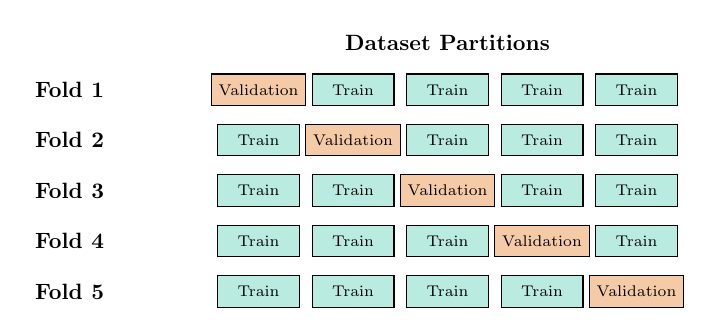
\begin{tikzpicture}[scale=0.8, every node/.style={transform shape}]
    \foreach \fold in {1,...,5} {
      \node at (-1.5, 3-\fold*0.8) {\textbf{Fold \fold}};
      \foreach \part in {1,...,5} {
        \ifnum\fold=\part
          \node[draw, fill=accent!40, minimum width=1.3cm, minimum height=0.5cm] at (\part*1.5, 3-\fold*0.8) {\scriptsize Validation};
        \else
          \node[draw, fill=primary!30, minimum width=1.3cm, minimum height=0.5cm] at (\part*1.5, 3-\fold*0.8) {\scriptsize Train};
        \fi
      }
    }
    \node[above] at (4.5, 2.7) {\textbf{Dataset Partitions}};
  \end{tikzpicture}
  \vfill
\end{frame}

% Slide 37: Grid Search Optimization: GridSearchCV
\begin{frame}{Grid Search Optimization: GridSearchCV}
  To find the best combination of multiple hyperparameters, we perform a \textbf{Grid Search}:
  \begin{itemize}
    \item We define a grid of values for each hyperparameter:
      \begin{align*}
        \text{hidden\_layer\_sizes} &\in \{\mathbf{H}_1 = (32, 16), \, \mathbf{H}_2 = (64, 32)\} \\
        \text{activation} &\in \{f_1 = \text{'relu'}, \, f_2 = \text{'tanh'}\} \\
        \text{alpha} &\in \{\alpha_1 = 0.01, \, \alpha_2 = 0.1\}
      \end{align*}
    \item The search space is the Cartesian product of these sets, yielding $2 \times 2 \times 2 = 8$ configurations.
    \item For each configuration, we run 5-Fold Cross-Validation. This requires training:
      $$8 \text{ configurations} \times 5 \text{ folds} = 40 \text{ training runs}$$
    \item The configuration with the highest averaged validation score (e.g., Macro F1) is selected as the best estimator and retrained on the entire training set.
  \end{itemize}
\end{frame}

% Module 6 Header
\begin{frame}[plain]
  \vfill
  \centering
  \begin{beamercolorbox}[sep=8pt,center,shadow=true,rounded=true]{palette primary}
    \usebeamerfont{title}\textbf{Module 6: Model Diagnostics \& Interpretability}
  \end{beamercolorbox}
  \vfill
\end{frame}

% Slide 39: Multiclass Diagnostics: Confusion Matrix
\begin{frame}{Multiclass Diagnostics: Confusion Matrix}
  A \textbf{Confusion Matrix} is a diagnostic contingency table that shows where classification errors occur:
  \begin{columns}
    \begin{column}{0.5\textwidth}
      \begin{itemize}
        \item **Rows:** Represent the actual true classes.
        \item **Columns:** Represent the model's predicted classes.
        \item **Diagonal Elements:** Represent correct predictions (True Positives).
        \item **Off-Diagonal Elements:** Highlight systematic errors (e.g., if Class 1: CC-SN is frequently misclassified as Class 2: Ia-SN).
      \end{itemize}
    \end{column}
    \begin{column}{0.5\textwidth}
      \begin{center}
        \begin{tabular}{c c c c}
          \toprule
          & \multicolumn{3}{c}{\textbf{Predicted Label}} \\
          \textbf{True Label} & Background & CC-SN & Ia-SN \\
          \midrule
          Background & \textbf{40} & 3 & 2 \\
          CC-SN & 2 & \textbf{6} & 1 \\
          Ia-SN & 1 & 1 & \textbf{4} \\
          \bottomrule
        \end{tabular}
      \end{center}
      In this example table, the model correctly predicted 40 background galaxies, 6 CC-SNe hosts, and 4 Ia-SNe hosts.
    \end{column}
  \end{columns}
\end{frame}

% Slide 40: Multiclass Diagnostics: One-vs-Rest ROC & AUC
\begin{frame}{Multiclass Diagnostics: One-vs-Rest ROC \& AUC}
  The Receiver Operating Characteristic (ROC) curve evaluates a classifier's sensitivity across different probability thresholds. For multiclass problems, we use the \textbf{One-vs-Rest (OvR)} method:
  \begin{itemize}
    \item We treat class $c$ as the positive class, and group all other classes together as the negative class. We plot:
      $$\text{True Positive Rate (TPR)} = \frac{\text{TP}}{\text{TP} + \text{FN}} \quad \text{vs.} \quad \text{False Positive Rate (FPR)} = \frac{\text{FP}}{\text{FP} + \text{TN}}$$
    \item We repeat this for each of the $C$ classes, generating $C$ separate ROC curves.
    \item \textbf{Area Under the Curve (AUC):} Integrates the area under the ROC curve:
      \begin{itemize}
        \item $\text{AUC} = 0.5$ represents a random guess classifier.
        \item $\text{AUC} = 1.0$ represents a perfect classifier.
      \end{itemize}
  \end{itemize}
\end{frame}

% Slide 41: Model Interpretability: The Black Box Challenge
\begin{frame}{Model Interpretability: The Black Box Challenge}
  In physics and astronomy, we do not just care about making accurate predictions; we must understand **why** the model made a prediction (what physical features it prioritized).
  \begin{itemize}
    \item In linear models (like linear regression), we can interpret weights directly:
      $$y = w_1 x_1 + w_2 x_2 \implies w_i \text{ is the direct sensitivity.}$$
    \item In an MLP, features are passed through multiple layers of matrix multiplications and non-linear activations:
      $$\mathbf{z}^{(L)} = \mathbf{W}^{(3)} f \left( \mathbf{W}^{(2)} f \left( \mathbf{W}^{(1)} \mathbf{x} + \mathbf{b}^{(1)} \right) + \mathbf{b}^{(2)} \right) + \mathbf{b}^{(3)}$$
    \item Because the inputs are blended across hidden layers, we cannot interpret individual weights. The model acts as a \textbf{black box}.
    \item We resolve this using \textbf{Permutation Feature Importance}.
  \end{itemize}
\end{frame}

% Slide 42: Permutation Feature Importance Theory
\begin{frame}{Permutation Feature Importance Theory}
  Let $M$ be a trained classifier, $D = (\mathbf{X}, \mathbf{y})$ be the validation dataset, and $s$ be the baseline score (e.g., Macro F1-score).
  \begin{block}{Breiman's Algorithm (2001)}
    For each physical feature $j$ (e.g., Star Formation Rate):
    \begin{enumerate}
      \item **Shuffle Column:** Randomly shuffle the values of column $j$ across the dataset. This breaks the physical correlation between feature $j$ and the target label $y$ while preserving the feature's distribution.
      \item **Evaluate:** Calculate the model performance $s^{(j)}$ on this perturbed dataset.
      \item **Compute Drop:** Define importance as the drop in performance:
        $$I(j) = s - s^{(j)}$$
    \end{enumerate}
  \end{block}
  \begin{itemize}
    \item If a feature is **critical**, shuffling it will degrade model performance, yielding a large $I(j) > 0$.
    \item If a feature is **irrelevant**, shuffling it has little effect, yielding $I(j) \approx 0$.
  \end{itemize}
\end{frame}

% Slide 43: Summary \& Best Practices
\begin{frame}{Summary \& Best Practices}
  When building classifiers for physical datasets, follow these rules:
  \begin{block}{The Machine Learning Checklist}
    \begin{description}
      \item[1. Scale features safely:] Center and scale inputs using Standardization. Only fit the scaler on the training set to prevent data leakage.
      \item[2. Split before oversampling:] Oversample training data only. Oversampling the validation/test set introduces leakage and yields artificially perfect metrics.
      \item[3. Stratify splits:] Always stratify train-test splits for imbalanced datasets.
      \item[4. Evaluate with Macro F1:] Do not rely on accuracy for imbalanced datasets. Use Macro F1 to weight rare classes equally.
      \item[5. Interpret black-box models:] Use Permutation Feature Importance to verify that the network learns physically meaningful correlations.
    \end{description}
  \end{block}
\end{frame}

\end{document}
